\chapter{Исследовательская часть}
\section{Технические характеристики}
Замеры производились на плате SMT32767 Nuckeo-144.

\begin{enumerate}
	\item Ядро: ARM Cortex M7, 216 МГц.
	\item SRAM: 516 Мб.
\end{enumerate}

При замерах времени ноутбук был включен в сеть электропитания.

\section{Демонстрация работы программы}
На рисунке \ref{img:demonstration} представлена демонстрация работы разработанной программы, показаны результаты вычислений расстояний Дамерау--Левенштейна и Левенштейна между словами <<claps>>,<<shmaps>>.
\clearpage
\begin{figure}[H]
	\centering
	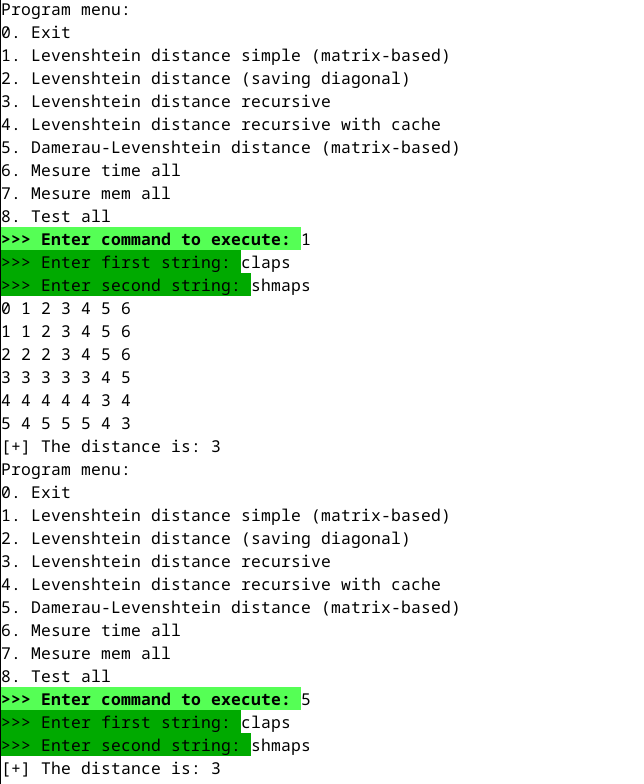
\includegraphics[height=0.5\textheight]{inc/img/work.png}
	\caption{Демонстрация работы программы}
	\label{img:demonstration}
\end{figure}

\clearpage

\section{Временные характеристики}

Результаты исследования замеров по времени приведены в таблице \ref{t:timings}.
Введем следующие обозначения для чтения таблиц:
\begin{enumerate}
	\item N~---~длина анализируемых строк;
	\item Lev~---~реализация алгоритма поиска расстояния Левенштейна с использованием матрицы;
	\item LevRec~---~рекурсивная реализация алгоритма поиска расстояния Левенштейна;
	\item LevRecCache~---~рекурсивная реализация алгоритма поиска расстояния Левенштейна с кешированием;
	\item DavLev~---~реализация алгоритма поиска расстояния Левенштейна с использованием матрицы.
\end{enumerate}

Ввиду того, что рекурсивная реализация алгоритма поиска расстояния Левенштейна работает медленнее, чем остальные рассматриваемые алгоритмы, замеры времени для этого алгоритма проводились с меньшим размером строк~---~до 9 включительно. Поэтому поля со значениями N большими 9 в соответствующем столбце помечены символом <<$\sim$>>. 

Замеры проводились на одинаковых длинах строк от 1 до 200 с различным шагом, для получения достоверных результатов замеры времени для каждой пары строк проводились 500 раз, после чего усреднялись. Все результаты вычислений приведены в миллисекундах.

\begin{table}[!ht]
	\centering
	\caption{Полученная таблица замеров по времени различных реализаций алгоритмов поиска редакционных расстояний}
	\begin{tabular}{|c|c|c|c|c|}
		\hline
		N  & Lev, мс & LevRec, мс & LevRecCache, мс & DavLev, мс \\
		\hline
		1 & 0.421872 & 0.212058 & 0.434712 & 0.430570 \\ \hline
		2 & 0.920052 & 0.454792 & 0.985639 & 0.951776 \\ \hline
		3 & 1.488031 & 0.817632 & 1.632186 & 1.540757 \\ \hline
		4 & 2.223468 & 1.925257 & 2.530816 & 2.303668 \\ \hline
		5 & 3.094647 & 6.637956 & 3.683479 & 3.221083 \\ \hline
		6 & 4.116389 & 30.511409 & 5.128874 & 4.295244 \\ \hline
		7 & 5.247164 & 157.772385 & 6.826485 & 5.525318 \\ \hline
		8 & 6.550792 & 868.326182 & 8.960211 & 6.997226 \\ \hline
		9 & 7.516181 & 3202.834432 & 10.706352 & 8.143731 \\ \hline
		10 & 8.517063 & $\sim$ & 13.000968 & 9.646358 \\ \hline
		11 & 9.464969 & $\sim$ & 14.645064 & 10.688708 \\ \hline
		12 & 10.530529 & $\sim$ & 16.548302 & 11.843978 \\ \hline
		13 & 11.726358 & $\sim$ & 18.775938 & 13.153469 \\ \hline
		14 & 13.158860 & $\sim$ & 21.463306 & 14.769491 \\ \hline
		15 & 14.847643 & $\sim$ & 24.322062 & 16.634343 \\ \hline
		20 & 17.395396 & $\sim$ & 29.600813 & 19.511076 \\ \hline
		25 & 21.025973 & $\sim$ & 37.099425 & 23.631597 \\ \hline
		30 & 25.873473 & $\sim$ & 47.847719 & 29.183306 \\ \hline
		35 & 32.227282 & $\sim$ & 62.292578 & 36.537368 \\ \hline
		40 & 40.211209 & $\sim$ & 81.158329 & 45.950269 \\ \hline
		45 & 49.829237 & $\sim$ & 103.791571 & 57.405801 \\ \hline
		50 & 61.352249 & $\sim$ & 131.034225 & 71.422056 \\ \hline
		100 & 103.502865 & $\sim$ & 241.415583 & 122.918591 \\ \hline
		150 & 203.208681 & $\sim$ & 482.096092 & 250.690342 \\ \hline
		200 & 387.066722 & $\sim$ & 914.509071 & 478.088641 \\ \hline	
	\end{tabular}
	\label{t:timings}
\end{table}
\clearpage
Приведенные  графики \ref{plt:time_matrix_cmp}--\ref{plt:time_mat_rec_cmp}  получены при помощи анализа данных таблицы \ref{t:timings}.
\begin{figure}[H]
	\centering
	\includesvg{inc/img/linear_cmp.svg}
	\caption{Сравнение по времени линейных реализаций алгоритмов поиска расстояний Левенштейна и Дамерау---Левенштейна}
	\label{plt:time_matrix_cmp}
\end{figure}

\begin{figure}[H]
	\centering
	\includesvg{inc/img/rec_cmp.svg}
	\caption{Сравнение по времени реализации рекурсивного поиска расстояния Левенштейна с кешированием и без}
	\label{plt:time_rec_cmp}
\end{figure}

\begin{figure}[H]
	\centering
	\includesvg{inc/img/lev_rec_cache_not_rec.svg}
	\caption{Сравнение по времени реализации рекурсивного с кешированием и линейного поиска расстояния Левенштейна}
	\label{plt:time_mat_rec_cmp}
\end{figure}

\section{Характеристики по памяти}
\begin{table}[!ht]
	\centering
	\caption{Полученная таблица замеров по памяти различных реализаций алгоритмов поиска редакционных расстояний}
	\begin{tabular}{|c|c|c|c|c|}
		\hline
		N  & Lev, байт & LevRec, байт & LevRecCache, байт & DavLev, байт \\
		1 & 144 & 416 & 528 & 144 \\ \hline
		2 & 184 & 592 & 640 & 184 \\ \hline
		3 & 240 & 768 & 1776 & 240 \\ \hline
		4 & 312 & 944 & 1284 & 312 \\ \hline
		5 & 400 & 1120 & 1024 & 400 \\ \hline
		6 & 504 & 1296 & 1828 & 504 \\ \hline
		7 & 624 & 1472 & 2112 & 624 \\ \hline
		8 & 760 & 1648 & 2404 & 760 \\ \hline
		9 & 912 & 1824 & 2704 & 912 \\ \hline
		10 & 1080 & $\sim$ & 3012 & 1080 \\ \hline
		11 & 1264 & $\sim$ & 3328 & 1264 \\ \hline
		12 & 1464 & $\sim$ & 3652 & 1464 \\ \hline
		13 & 1680 & $\sim$ & 3984 & 1680 \\ \hline
		14 & 1912 & $\sim$ & 4324 & 1912 \\ \hline
		15 & 2160 & $\sim$ & 4672 & 2160 \\ \hline
		20 & 3640 & $\sim$ & 6532 & 3640 \\ \hline
		25 & 5520 & $\sim$ & 8592 & 5520 \\ \hline
		30 & 7800 & $\sim$ & 10852 & 7800 \\ \hline
		35 & 10480 & $\sim$ & 13312 & 10480 \\ \hline
		40 & 13560 & $\sim$ & 15972 & 13560 \\ \hline
		45 & 17040 & $\sim$ & 18832 & 17040 \\ \hline
		50 & 20920 & $\sim$ & 21892 & 20920 \\ \hline
		100 & 81720 & $\sim$ & 63492 & 81720 \\ \hline
		150 & 182520 & $\sim$ & 125092 & 182520 \\ \hline
		200 & 323320 & $\sim$ & 206692 & 323320 \\ \hline
	\end{tabular}
	\label{t:memory}
\end{table}

\begin{figure}[H]
	\centering
	\includesvg{inc/img/rec_mem_cmp.svg}
	\caption{Сравнение по памяти реализации рекурсивного поиска расстояния Левенштейна с кешированием и без}
	\label{plt:memory_mat_rec}
\end{figure}

\begin{figure}[H]
	\centering
	\includesvg{inc/img/lev_rec_cache_not_rec_mem.svg}
	\caption{Сравнение по памяти реализации рекурсивного с кешированием и линейного поиска расстояния Левенштейна}
	\label{plt:memory_rec}
\end{figure}

\clearpage

\section{Результаты анализа различных реализаций}

\subsection{Сравнение по времени исполнения}
Замеры показали, что линейный алгоритм поиска расстояния Левенштейна работает быстрее линейного алгоритма поиска расстояния Дамерау-Левенштейна в $\sim$1.235 раз. Это обусловлено тем, что помимо всех действий, выполняемых первым упомянутым алгоритмом, необходимо также учесть операцию транспонирования.

Также замеры показали, что рекурсивная реализация алгоритма Левенштейнва с кешированием работает значительно быстрее (в $\sim$299.15 раз), чем без кеширования. Это обусловлено тем, что в первом упомянотом алгоритме за счет кеширования операции вычисления значения расстояния на каждом шаге рекурсии не выполняются повторно.

По полученным данным также видно, что рекурсивная реализация алгоритма линейного поиска с кешированием медленнее линейной реализаци в $\sim$2.36 раз.

\subsection{Сравнение затраченной памяти}

Анализ таблицы \ref{t:memory} показал, что по расходу памяти линейные алгоритмы проигрывают рекурсивным: максимальный размер используемой памяти в линейном алгоритме растет как произведение длин строк, в то время как в рекурсивном алгоритме~---~как сумма длин строк.
При малых длинах слов рекурсивные алгоритмы уступают линейным, это обусловлено большим количеством вспомогательных переменных в реализации рекурсивного алгоритма. Наиболее эффективным по памяти является рекурсивная реализация алгоритма поиска расстояния Левенштейна.
Также линейные алгоритмы поиска расстояния Левенштейна и Дамерау-Левенштейна показали одинаковые результаты по памяти. Это связано с схожестю алгоритмов и отсутствием во втором упомянутом алгоритме дополнительных переменных по сравнению с первым.